\documentclass[a4paper]{article}

\usepackage[utf8]{inputenc}
\usepackage[T1]{fontenc}
\usepackage{graphicx}
\usepackage{hyperref}
\usepackage{amsmath}
\usepackage{amssymb}
\usepackage{amsthm}
\usepackage{mathenv}
\usepackage{multirow}
\usepackage{fullpage}

\DeclareMathAlphabet{\itbf}{OML}{cmm}{b}{it}

% numérotation au sein de chaque section (du style "2.1")
\numberwithin{equation}{section}

% commandes perso
\newcommand{\R}{\mathbb{R}}
\newcommand{\ie}{\emph{i.e.} }
\newcommand{\RnX}{\mathbb{R}_n[X]}
\newcommand{\N}{\mathbb{N}}
\newcommand{\C}{\mathcal{C}}
\newcommand{\Ccinf}{\mathcal{C}_c^{\infty}}
\newcommand{\Cinf}{\mathcal{C}^{\infty}}
\newcommand{\supp}{\textrm{supp}}
\newcommand{\bx}{\mathbf{x}}
\newtheorem{definition}{Definition}
\newtheorem{lemma}{Lemma}
\newtheorem{theorem}{Theorem}

\title{Consistency of Fanbeam Projections of a Translating Object Along an Arc of a Circle}
\author{}
\date{}

\begin{document}

\maketitle

\begin{abstract}
This note aims at extending the results of~\cite{clackdoyle2015consistency} to the case of a translating object.
\end{abstract}

\section{Introduction}

\section{Theory} 
\label{sec:theory}

\subsection{Problem under consideration}
\label{sub:problem_under_consideration}

Let us begin with some notations and definitions. We will consider an object in $\R^2$ to be imaged by a fanbeam source that follows an arc of circle with center $O$ and radius $R_0$ (see Figure~\ref{fig:notations}, left). The object will be identified with its density function $\mathbf{x} \mapsto \mu(\mathbf{x}) \in \Ccinf(\R^2)$.
\begin{figure}[!ht]
	\centering
	\begin{tabular}{cc}
	\includegraphics[width=8cm]{figs/frame_scanner_still.eps} &
	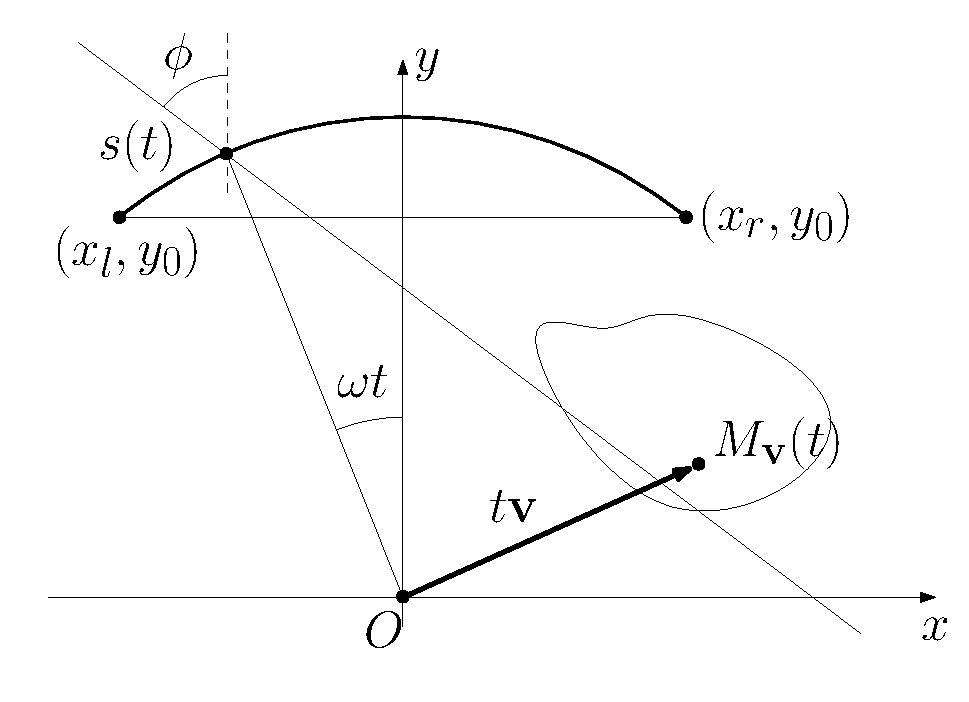
\includegraphics[width=8cm]{figs/frame_scanner.eps}
	\end{tabular}
	\caption{Problem under consideration. The source point $s(t)$ follows the arc of circle depicted in bold. This latter has center $O$ and radius $R_0$.\label{fig:notations}}
\end{figure}
The angular velocity of the source will be denoted $\omega$, and the time $t$ will range from $-T/2$ to $T/2$, where $T>0$. Hence, if we denote $s(t)$ the position of the source at time $t$, one has
\begin{equation}
	s(t) = \left( -R_0 \sin(\omega t), R_0 \cos(\omega t) \right).
\label{eq:source_position}
\end{equation}
Furthermore, we will denote $s(T/2)=(x_l,y_l)$ (resp. $s(-T/2)=(x_r,y_r)$) the extreme left (resp. right) position of the source. Since $y_l = y_r = R_0 \cos(\omega T/2)$, we will call $y_0$ this common value. In the following, we will suppose that $\supp(\mu)$ lies in the half-space $\{ y < y_0 \}$, and that $y_0 > 0$ (\ie $0 < \omega T < \pi$).

We will suppose that at any time $t$ rays are simultaneously emitted from the source $s(t)$ with angle $\phi$ ranging from $-\pi/2$ to $\pi/2$. With this setup in mind, we can define the operator giving the acquired data from the object.
\begin{definition}
The \emph{fanbeam projection data} of an object with density function $\mu$ is a function $(t,\phi) \mapsto T\mu(t,\phi)$ defined by
\begin{equation}
	(T\mu)(t,\phi) = \int_0^{+\infty} \mu \left( s(t) + l \left[ \sin \phi, -\cos \phi \right] \right) dl,
\end{equation}
where $t \in \left[ -T/2, T/2\right]$, $\phi \in \left[ -\pi/2, \pi/2\right]$ and $s(t)$ is given by~(\ref{eq:source_position}). The operator $\mu \mapsto T\mu$ is called the \emph{fanbeam projection operator}.
\end{definition}


Now let us suppose that the object is translating along the $x$-axis with a constant velocity $v \in \R$ (see Figure~\ref{fig:notations}, right). In other words, if we denote $M(t)$ its center of mass at any time $t$, we have
\begin{equation}
	M_v(t) =  \left( \left( t + \frac{T}{2} \right)v, 0 \right).
\label{eq:center_of_mass}
\end{equation}
The density function of the object now depends on both the space variable $\bx \in \R^2$ and the time $t$. If we denote it $\mu_v$, we have
\begin{equation}
	\mu_v(t,\bx) = \mu\left( \bx - M_v(t)\right).
\end{equation}
In this regard, the fanbeam projection data will be modified in the following way.
\begin{definition}
The \emph{fanbeam projection data of a translating object} with density function $\mu$ and translating velocity $v$ is given by
\begin{equation}
	(T_v\mu)(t,\phi) = \left( T \mu_v(t,\cdot) \right)(t,\phi).
\label{eq:def_Tv}
\end{equation}
\end{definition}

The aim of this note is to derive data consistency conditions (DCCs) from~(\ref{eq:def_Tv}), in order to retrieve the velocity $v$.

\subsection{Derivation of DCCs}

In order to derive DCCs, we will first change our frame of reference, from $\left(O, x, y\right)$ to $\left(M(t), x, y\right)$, so that the object is at the center. In this frame, the coordinates of the source are given by $s_v(t)=s(t)-M_v(t)$, so that we have
\begin{equation}
	(T_v\mu)(t,\phi) = \int_0^{+\infty} \mu \left( s_v(t) + l \left[ \sin \phi, -\cos \phi \right] \right) dl.
\end{equation}
In other words, we are now dealing with a fixed object illuminated by a source following an arc of a cycloid (see Figure~\ref{fig:change_frame}).
\begin{figure}[!ht]
	\centering
	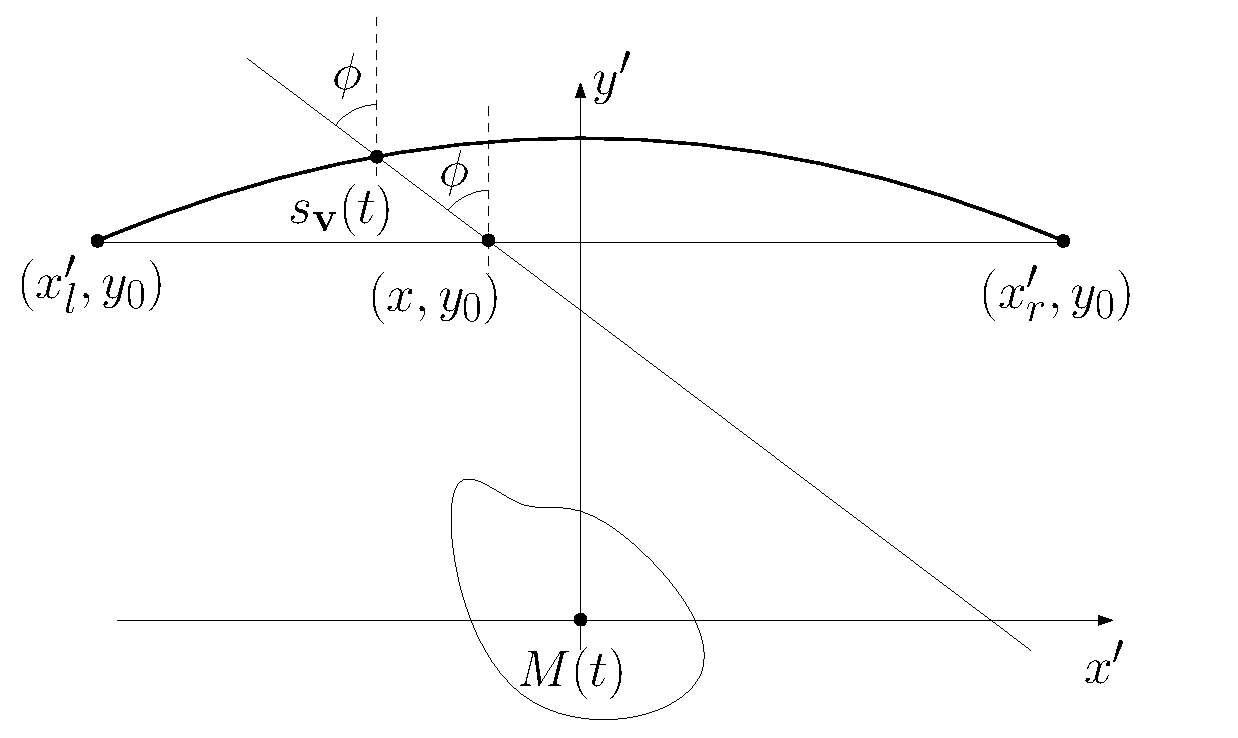
\includegraphics[width=12cm]{figs/frame_object.eps}
	\caption{Change of frame: the object is now at center of the coordinates system.\label{fig:change_frame}}
\end{figure}

For any time $t$, let us denote the coordinates of $s_v(t)$ by $\left( s_{1,v}(t), s_{2,v}(t) \right)$. Here, the extreme points $s_v(-T/2)$ and $s_v(T/2)$ have the same $y$-coordinate $y_0$, and $s_{1,v}(-T/2)=x_r$, but $s_{1,v}(T/2)$ differs. We will call it $x'_l$; note that one has $x'_l = x_l - Tv$.
This allows us to define what we call the \emph{virtual fanbeam projection} from a point $(x,y_0)$.
\begin{definition}
	For any point $x$ between $x'_l$ and $x_r$, for any angle $\phi \in \left[ -\pi/2, \pi/2\right]$, the \emph{virtual fanbeam projection} of the object $\mu$ is defined by
\begin{equation}
	\left( \tilde{T}\mu	\right)(x,\phi) = \int_0^{+\infty} \mu \left( (x,y_0) + l \left[ \sin \phi, -\cos \phi \right] \right) dl.
\end{equation}
This is called \emph{virtual} since it does not correspond to an actual position of the source.
\end{definition}

In the following lemma, we will make a connection between the virtual fanbeam projection and the fanbeam projection of the translating object.
\begin{lemma}
	Let us fix a time $t \in \left[ -T/2, T/2\right]$ and an angle $\phi \in \left[ -\pi/2, \pi/2\right]$. Let us define
	\begin{equation}
		x = s_{1,v}(t) + \tan \phi \left( s_{2,v}(t) - y_0 \right).
	\end{equation}
	Then, one has
	\begin{equation}
		\left( \tilde{T}\mu	\right)(x,\phi) = \left( T_v\mu	\right)(t,\phi).
	\end{equation}
\label{lem:T_x_t}
\end{lemma}
\begin{proof}
The idea is that the point $(x,y_0)$ is the intersection between the line $\{y=y_0\}$ and the ray coming from $s_v(t)$ with angle $\phi$ (see Figure~\ref{fig:change_frame}). Since $\supp(\mu)$ is under the line $\{ y=y_0 \}$, the integral does not differ if we start from $(x,y_0)$ or from $s_v(t)$. Indeed, one has
\begin{equation}
	\int_0^{+\infty} \mu \left( (x,y_0) + l \left[ \sin \phi, -\cos \phi \right] \right) dl = \int_{-\infty}^{+\infty} \mu \left( (x,y_0) + l \left[ \sin \phi, -\cos \phi \right] \right) dl.
\end{equation}
Let us now perform the following change of variable
\begin{equation}
	l' \leftrightarrow l + \frac{s_{2,v}(t) - y_0}{\cos \phi}.
\end{equation}
By definition of $x$, it gives $x + l \sin \phi = s_{1,v}(t) + l' \sin \phi$ and $y_0 - l \cos \phi = s_{2,v}(t) - l' \cos \phi$. We then have
\begin{equation}
	\int_{-\infty}^{+\infty} \mu \left( (x,y_0) + l \left[ \sin \phi, -\cos \phi \right] \right) dl = \int_{-\infty}^{+\infty} \mu \left( s_v(t) + l' \left[ \sin \phi, -\cos \phi \right] \right) dl'.
\end{equation}
Restricting the domain of integration from $l'=0$ to $t = + \infty$ then leads us to the desired result.
\end{proof}

We can now define what are the DCCs of our problem.
\begin{theorem}
Let us fix a density function $\mu$. For any integer $n$, there exist a function $(x,t)\mapsto W_{n,v}(t,x) \in \Cinf \left( [-T/2,T/2] \times [x'_l,x_r] \right)$ such that
\begin{equation}
	B_n := x \mapsto \int_{-T/2}^{T/2} \left( T_v \mu \right)\left( t,\lambda(t) \right) W_n(x,t,v) dt \in \RnX,
\label{eq:DCC}
\end{equation}
where $\lambda(t)$ is defined by
\begin{equation}
	\lambda_t = \arctan \left( \frac{x + R_0 \sin(\omega t) + \left( t + \frac{T}{2} \right)v}{R_0 \cos(\omega t) - y_0} \right).
\end{equation}
Moreover, it is possible to derive $W_{n,v}(t,x)$ analytically.
\end{theorem}
\begin{proof}
The DCCs derived in~\cite{clackdoyle2015consistency} heavily rely on a relation between $\tan \phi$ and the angle $\omega t$ (see Figure~\ref{fig:notations}). This relation is then differentiated to change variables into the integral in~(\ref{eq:DCC}), which gives the following expression, known to be a polynom according to~\cite{clackdoyle2013necessary}
\begin{equation}
	\int_{-\pi/2}^{\pi/2}  \left( \tilde{T}\mu	\right)(x,\phi) \frac{\tan^n \phi}{\cos \phi} d\phi.
\end{equation}

We will follow the same path here. First, the formula giving $\tan \phi$ is nearly the same as in~\cite{clackdoyle2015consistency},~\emph{i.e.}
$$
\tan \phi = \frac{x + R_0 \sin(\omega t) + \left( t + \frac{T}{2} \right)v}{R_0 \cos(\omega t) - y_0}.
$$
Then, taking its derivative allows us to write the Jacobian for a change of variables from $\phi$ to $t$
\begin{align*}
\frac{d\phi}{\cos^2 \phi} &= \frac{ \left( R_0 \omega \cos(\omega t) +v \right) \left( R_0 \cos(\omega t) - y_0 \right) + R_0 \omega \sin(\omega t) \left( x + R_0 \sin(\omega t) + \left( t + \frac{T}{2} \right)v \right) }{ \left( R_0 \cos(\omega t) - y_0 \right)^2 } dt \\
 &= \frac{ R_0^2 \omega - v y_0 + R_0 \cos(\omega t)(v-\omega y_0) + R_0 \omega \sin(\omega t)(x + \left( t + \frac{T}{2} \right)v ) }{ \left( R_0 \cos(\omega t) - y_0 \right)^2 } dt\\
 &:= J(x,t,v) dt.
\end{align*}
Hence, one can write
\begin{align}
	\frac{\tan^n \phi}{\cos \phi} d\phi &= \tan^n \phi \cos \phi \frac{d\phi}{\cos^2 \phi} \\
	&= \frac{ \left( x+R_0 \sin(\omega t) + \left( t + \frac{T}{2} \right)v \right)^n }{D_{x,t} \left( R_0 \cos(\omega t) - y_0 \right)^{n-1}} J(x,t,v) dt \label{eq:Dxt_first_occurence} \\
	&:= W_n(x,t,v) dt,
\end{align}
where the term $D_{x,t}$ in equation~(\ref{eq:Dxt_first_occurence}) refers to the distance between the source point $s_v(t)$ and the virtual point $(x,y_0)$.

With the help of lemma~\ref{lem:T_x_t}, the change of variable from $t$ to $\phi$ then leads us to
\begin{equation}
	B_n(x) = \int_{-\pi/2}^{\pi/2}  \left( \tilde{T}\mu	\right)(x,\phi) \frac{\tan^n \phi}{\cos \phi} d\phi,
\end{equation}
which is known to be a polynom of degree at most $n$ according to~\cite{clackdoyle2013necessary} as mentioned above.
\end{proof}

\section{Numerical simulations}

Let us suppose that we have the projections $g(x,\phi)$. In order to recover $v$, we can perform the following optimization procedure. Since $B_n(x)$ in equation~(\ref{eq:DCC}) is supposed to be a polynom of order $\leq n$, one can minimize
\begin{equation}
	\mathcal{J}(v) = \sum_n \Vert \textrm{res} \left( B_n(x,v) \right) \Vert^2
\end{equation}
with respect to $v$, where $\textrm{res}$ is the residual of the projection onto $\R_n[X]$. The minimization procedure can be done using the gradient of $\mathcal{J}(v)$, given by
\begin{equation}
	\nabla \mathcal{J}(v) = 2 \sum_n B_n(x,v) \int_{-T/2}^{T/2} g(t,\phi) \frac{\partial W_n}{\partial v}(x,t,v) dt.
\end{equation}

\bibliographystyle{plain}
\bibliography{DCC_translation}

\end{document}

